
\newpage
\setlength{\voffset}{-3cm}

\begin{center}
\section{\textbf{\huge{User Handling}}}

\Large{Use Cases}
\end{center}

%--------START EDITING HERE FOR HANDLING---------
%Maria

%--------USER LOGIN---------
\subsection{User login}
\textbf{Description:}
This use-case enables a user to log into the system so as to insert medical data.
\subsubsection{Prioritization:}
Critical
\subsubsection{Conditions and Data Structures:}
\textbf{Pre-Conditions:}
\begin{itemize}
	\item , The user must be found on LDAP, thus have a valid username and password.
	\item The user must not already be logged in.
\end{itemize}

\textbf{Post-Conditions:}	
\begin{itemize}
	\item The user is loged in.
	\item The user is authenticated.
	\item The user can carry out system activities.
\end{itemize}
\subsubsection{Required Functionality:} 
\subsubsection{Process Specifications:} 

%\textbf{Use case diagram for Login}\\
%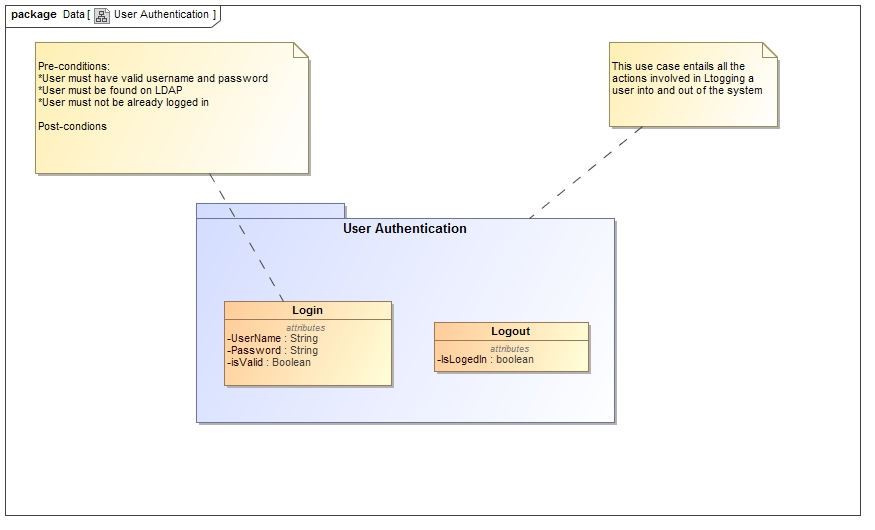
\includegraphics[width=1\linewidth]{./Images/Author/Login.jpg}\\
\left( 

%--------USER LOGOUT---------
\subsection{Logout}
\textbf{Description:}
\subsubsection{Prioritization:}
\subsubsection{Conditions and Data Structures:}
\textbf{Pre-Conditions:}
\textbf{Post-Conditions:}	
\subsubsection{Required Functionality:} 
\subsubsection{Process Specifications:}



%--------USER AUTHENTICATION---------
\subsection{User Authorization}
\textbf{Description:}
\subsubsection{Prioritization:}
\subsubsection{Conditions and Data Structures:}
\textbf{Pre-Conditions:}
\textbf{Post-Conditions:}	
\subsubsection{Required Functionality:} 
\subsubsection{Process Specifications:}